%%%%%%%%%%%%%%%%%%%%%%%%%%%%%%%%%%%%%%%%%%%%%%%%
%% Intro to LaTeX and Template for Homework Assignments
%% Quantitative Methods in Political Science
%% University of Mannheim
%% Fall 2018
%%%%%%%%%%%%%%%%%%%%%%%%%%%%%%%%%%%%%%%%%%%%%%%%

% created by Marcel Neunhoeffer & Sebastian Sternberg


% This template and tutorial will help you to write up your homework. It will also help you to use Latex for other assignments than this course's homework.

%%%%%%%%%%%%%%%%%%%%%%%%%%%%%%%%%%%%%%%%%%%%%%%%
% Before we get started
%%%%%%%%%%%%%%%%%%%%%%%%%%%%%%%%%%%%%%%%%%%%%%%%

% Make an account on overleaf.com and get started. No need to install anything.

%%%%%%%%%%%%%%%%%%%%%%%%%%%%%%%%%%%%%%%%%%%%%%%%
% Or if you want it the nerdy way...
% INSTALL LATEX: Before we can get started you need to install LaTeX on your computer.
				% Windows: http://miktex.org/download
				% Mac:         http://www.tug.org/mactex/mactex-download.html	
				% There a many more different LaTeX editors out there for both operating systems. I use TeXworks because it looks the same on Windows and Mac.
				

% SAVE THE FILE: The first thing you need to do is to save your LaTeX file in a directory as a .tex file. You will not be able to do anything else unless your file is saved. I suggest to save the .tex file in the same folder with your .R script and where you will save your plots from R to. Let's call this file template_homework1.tex and save it in your Week 1 folder.


% COMPILE THE FILE: After setting up your file, using your LaTeX editor (texmaker, texshop), you can compile your document using PDFLaTeX.
	% Compiling your file tells LaTeX to take the code you have written and create a pdf file
	% After compiling your file, in your directory will appear four new files, including a .pdf file. This is your output document.
	% It is good to compile your file regularly so that you can see how your code is translating into your document.
	
	
% ERRORS: If you get an error message, something is wrong in your code. Fix errors before they pile up!
	% As with error messages in R, google the exact error message if you have a question!
%%%%%%%%%%%%%%%%%%%%%%%%%%%%%%%%%%%%%%%%%%%%%%%%


% Now again for everyone...

% COMMANDS: 
	% To do anything in LaTeX, you must use commands
	% Commands tell LaTeX when to start your document, how you want your document to look, and how to format your document
	% Commands ALWAYS begin with a backslash \

% Everything following the % sign is a comment and will not be used by Latex to compile your document.
% This is very similar to # comments in R.

% Every .tex file usually consists of four parts.
% 1. Document Class
% 2. Packages
% 3. Header
% 4. Your Document

%%%%%%%%%%%%%%%%%%%%%%%%%%%%%%%%%%%%%%%%%%%%%%%%
% 1. Document Class
%%%%%%%%%%%%%%%%%%%%%%%%%%%%%%%%%%%%%%%%%%%%%%%%
 
 % The first command you will always have will declare your document class. This tells LaTeX what type of document you are creating (article, presentation, poster, etc). 
% \documentclass is the command
% in {} you specify the type of document
% in [] you define additional parameters
 
\documentclass[a4paper,12pt]{article} % This defines the style of your paper

% We usually use the article type. The additional parameters are the format of the paper you want to print it on and the standard font size. For us this is a4paper and 12pt.

%%%%%%%%%%%%%%%%%%%%%%%%%%%%%%%%%%%%%%%%%%%%%%%%
% 2. Packages
%%%%%%%%%%%%%%%%%%%%%%%%%%%%%%%%%%%%%%%%%%%%%%%%

% Packages are libraries of commands that LaTeX can call when compiling the document. With the specialized commands you can customize the formatting of your document.
% If the packages we call are not installed yet, TeXworks will ask you to install the necessary packages while compiling.

% First, we usually want to set the margins of our document. For this we use the package geometry. We call the package with the \usepackage command. The package goes in the {}, the parameters again go into the [].
\usepackage[top = 2.5cm, bottom = 2.5cm, left = 2.5cm, right = 2.5cm]{geometry} 

% Unfortunately, LaTeX has a hard time interpreting German Umlaute. The following two lines and packages should help. If it doesn't work for you please let me know.

% Configuración de idioma
\usepackage[T1]{fontenc}
\usepackage[utf8]{inputenc}

\usepackage[spanish]{babel}

% Paquete para la inserción de otro pdf
\usepackage[final]{pdfpages}

% Paquete para las expresiones matemáticas avanzadas
\usepackage{amsmath}

% Paquetes con complementos de símbolos
\usepackage{textcomp}

% Paquete para mostrar condicionalmente las soluciones en el PDF
\usepackage{etoolbox}

\newtoggle{answer}
\toggletrue{answer}
%\togglefalse{answer}


% Entorno para la numeración de las cuestiones
\newcounter{question}[section]
\newenvironment{question}{\refstepcounter{question} {\bfseries\thequestion}.\ }{}


% The following two packages - multirow and booktabs - are needed to create nice looking tables.
\usepackage{multirow} % Multirow is for tables with multiple rows within one cell.
\usepackage{booktabs} % For even nicer tables.

% As we usually want to include some plots (.pdf files) we need a package for that.
\usepackage{graphicx} 

% The default setting of LaTeX is to indent new paragraphs. This is useful for articles. But not really nice for homework problem sets. The following command sets the indent to 0.
\usepackage{setspace}
\setlength{\parindent}{0in}

% Package to place figures where you want them.
\usepackage{float}

% The fancyhdr package let's us create nice headers.
\usepackage{fancyhdr}

% The hyperref package let's us create web page links.
\usepackage[hidelinks]{hyperref}

%%%%%%%%%%%%%%%%%%%%%%%%%%%%%%%%%%%%%%%%%%%%%%%%
% 3. Header (and Footer)
%%%%%%%%%%%%%%%%%%%%%%%%%%%%%%%%%%%%%%%%%%%%%%%%

% To make our document nice we want a header and number the pages in the footer.

\pagestyle{fancy} % With this command we can customize the header style.

\fancyhf{} % This makes sure we do not have other information in our header or footer.

\lhead{\footnotesize Calibración Linac }% \lhead puts text in the top left corner. \footnotesize sets our font to a smaller size.

%\rhead works just like \lhead (you can also use \chead)
\rhead{\footnotesize Problema} %<---- Fill in your lastnames.

% Similar commands work for the footer (\lfoot, \cfoot and \rfoot).
% We want to put our page number in the center.
\cfoot{\footnotesize \thepage} 


%%%%%%%%%%%%%%%%%%%%%%%%%%%%%%%%%%%%%%%%%%%%%%%%
% 4. Your document
%%%%%%%%%%%%%%%%%%%%%%%%%%%%%%%%%%%%%%%%%%%%%%%%

% Now, you need to tell LaTeX where your document starts. We do this with the \begin{document} command.
% Like brackets every \begin{} command needs a corresponding \end{} command. We come back to this later.

\begin{document}
\renewcommand{\tablename}{Tabla}


%%%%%%%%%%%%%%%%%%%%%%%%%%%%%%%%%%%%%%%%%%%%%%%%
%%%%%%%%%%%%%%%%%%%%%%%%%%%%%%%%%%%%%%%%%%%%%%%%

%%%%%%%%%%%%%%%%%%%%%%%%%%%%%%%%%%%%%%%%%%%%%%%%
% Title section of the document
%%%%%%%%%%%%%%%%%%%%%%%%%%%%%%%%%%%%%%%%%%%%%%%%

% For the title section we want to reproduce the title section of the Problem Set and add your names.

\thispagestyle{empty} % This command disables the header on the first page. 

\begin{tabular}{p{11.2cm} r}  % This is a simple tabular environment to align your text nicely 
{\large \bf Física de la Radioterapia} & \multirow{2}{4cm}{\includegraphics[width=4cm]
{60-2016-09-20-Marca UCM Secundaria logo negro RGB.jpg}}\\
Máster en Física Biomédica & \\
\hline% \hline produces horizontal lines.
\\
\end{tabular} % Our tabular environment ends here.

\vspace*{0.3cm} % Now we want to add some vertical space in between the line and our title.

\begin{center} % Everything within the center environment is centered.
	{\Large \bf Calibración acelerador lineal} % <---- Don't forget to put in the right number
	\vspace{2mm}
	
        % YOUR NAMES GO HERE
	{} % <---- Fill in your names here!
		
\end{center}  

\vspace{0.4cm}

%%%%%%%%%%%%%%%%%%%%%%%%%%%%%%%%%%%%%%%%%%%%%%%%
%%%%%%%%%%%%%%%%%%%%%%%%%%%%%%%%%%%%%%%%%%%%%%%%

% Up until this point you only have to make minor changes for every week (Number of the homework). Your write up essentially starts here.

\textbf{Objetivo}.
Determinar la dosis absorbida producida por un campo de radiación en condiciones estándar de calibración en tres puntos de una cuba de agua utilizando medidas realizadas mediante una cámara de ionización tipo Farmer y aplicando el protocolo de dosimetría de la IAEA TRS398.

\textbf{Datos}.
El código de práctica TRS398 puede consultarse en el enlace:

\noindent \textbf{\url{https://www-pub.iaea.org/MTCD/publications/PDF/TRS_398s_Web.pdf}}

Los datos de la cámara empleada están recogidos en el certificado de calibración que se da anexo a este documento.

Previamente se ha determinado que para esta cámara los factores de corrección por saturación $k_{sat}$ y por polarización $k_{pol}$ son ambos igual a uno en las condiciones de medida consideradas.

La energía del haz empleado corresponde a una razón TPR${}_{20, 10} = 0.694$.

Para recolectar la carga producida en la cámara se utiliza un electrómetro con una resolución de $0.001$ nC.

Se realiza primero una medida sin radiación durante un minuto, registrándose en el electrómetro una carga acumulada de $0.078$ nC. A continuación, después de resetear el electrómetro, se programa el acelerador para que emita 200 UM empleando una tasa de 300 UM/min. El proceso se repite tres veces en cada uno de los puntos de medida.

Las lecturas del electrómetro tras cada irradiación son:

\begin{itemize}
    \item Punto A: $23.527$ nC, $23.332$ nC, y $23.291$ nC
    \item Punto B: $7.275$ nC, $7.322$ nC y $7.361$ nC
    \item Punto C: $0.192$ nC, $0.191$ nC y $0.191$ nC
\end{itemize}

Las condiciones ambientales son: $23.2$\textcelsius{} de temperatura y $935$ hPa de presión.

{\bf Cuestiones}.

\begin{question}
Obtener de los datos del TRS398 el factor de corrección de la calibración de la cámara por la energía para el haz utilizado.

    \iftoggle{answer}{
        {\bf Solución}. 
        Como en el certificado de calibración de la cámara la calidad del haz de referencia corresponde al ${}^{60}$Co, según el protocolo TRS398 podemos denotar el factor de corrección de la calibración por la energía $k_{Q, Q_0}$ como $k_Q$.
        
        El $k_Q$ se obtiene interpolando en la tabla correspondiente al modelo de cámara PTW 30013, página 85 CUADRO 14, usando el valor dado para el TPR${}_{20,10}$.
        
        \begin{center}
        \vspace{10pt}
        \begin{tabular}{ c c } 
        TPR${}_{20,10}$ & $k_Q$ \\
         \hline
         0.700 & 0.988 \\ 
         0.680 & 0.990 \\ 
         \textbf{0.694} & \textbf{0.9886} \\ 
         \hline
        \end{tabular}
        \vspace{10pt}
        \end{center}

    } % Final de la solución

\end{question}

\begin{question}
Determinar la dosis absorbida suministrada por el acelerador en cada punto de medida.

    \iftoggle{answer}{
        {\bf Solución}. 
        La dosis absorbida en agua para el haz considerado $D_{w, Q}$ se determinará según la expresión
        \begin{equation}
            D_{w, Q} = M_Q\;N_{D, w, Q_0}\;k_Q.
        \end{equation}
        
        El valor del factor de calibración de la cámara en condiciones de referencia se toma del certificado de calibración $N_{D, w, Q_0}  = 5.396\cdot 10^{-7}$ Gy/C.
        
        $M_Q$ es la lectura neta del electrómetro expresado en condiciones normales. 
        
        Para obtener la lectura neta, a la lectura bruta le tenemos que restar la contribución de las fugas. Las fugas se han determinado durante un minuto mientras que para completar las 200 UM de las medidas empleando una tasa de 300 UM/min se requieren 2/3 minutos. Asumiendo que las fugas se acumulan de forma constante en el tiempo, las fugas correspondientes al tiempo de irradiación serán $0.078$ nC/min $\cdot$ 2/3 minutos = $0.052$ nC.
        
        La lectura neta se corrige por el factor de presión y temperatura 
        
        \begin{equation}
            f_{p,T} = \frac{1013}{p} \cdot \frac{273.25+T}{293.25} = \frac{1013}{935} \cdot \frac{273.25+23.2}{293.25} = 1.096
        \end{equation}
        
        \noindent para llevarla a condiciones normales.
        
        Combinando todos estos resultados resulta
        
        \begin{equation}
            D_{w, Q} = (\bar L_p-0.052)\;\text{nC}\cdot 1.096\cdot 0.05396\;\text{Gy/nC}\cdot 0.9886
        \end{equation}
        
        \noindent donde $\bar L_p$ es el promedio de las tres lecturas realizadas en cada punto $p$.
        
        \begin{center}
        \vspace{10pt}
        \begin{tabular}{ c c c} 
        Punto & $\bar L_p$ (nC) & $D_{w,Q}$ (Gy)  \\
         \hline
         A &  23.383    & 1.364 \\ 
         B & 7.319      & 0.425 \\ 
         C & 0.191      & 0.008 \\
         \hline
        \end{tabular}
        \vspace{10pt}
        \end{center}
        
 
    } % Final de la solución

\end{question}

\begin{question}
Estimar la incertidumbre en la determinación de la dosis absorbida considerando la resolución del electrómetro, la incertidumbre del certificado de calibración y la repetibilidad de la medida. ¿En qué punto la incertidumbre relativa es mayor? ¿Y menor?

    \iftoggle{answer}{
        {\bf Solución}. 
        Para calcular la incertidumbre, tenemos que tomar en cuenta tres contribuciones:
        \begin{itemize}
            \item La incertidumbre estadística de cada medida individual (por fluctuaciones del acelerador, del electrómetro, fugas etc.) que estimamos como la desviación estándar de cada conjunto de tres medidas hechas en cada punto.
            \item La incertidumbre debida a la resolución del electrómetro. Esta se podría estimar como la mitad de la resolución ($0.0005$ nC), pero hay que tener en cuenta que afecta tanto a la medida bruta como a la medida de fugas. Por lo tanto, para calcular la incertidumbre de la lectura neta tomamos el doble de ese valor: $0.001$ nC.
            \item La incertidumbre del certificado de calibración, que viene dada como el $1.1$\% con un factor de cobertura $k=2$, correspondiente a dos desviaciones estándar. Tomaremos por tanto el valor del promedio obtenido y lo multiplicamos por $0.0055$.

        \end{itemize}
        
        Calculamos la incertidumbre de lectura $uM_Q$ como la suma cuadrática de las dos primeras contribuciones
        \begin{center}
        \vspace{10pt}
        \begin{tabular}{ c c c c} 
        Punto & $\sigma L_p$ (nC) & Resolución (nC) & $uM_Q$ (nC) \\
         \hline
         A	& 0.1261 &	0.0010	& 0.1261 \\
         B	& 0.0431 &  0.0010	& 0.0431 \\
         C	& 0.0006 &	0.0010	& 0.0012 \\
         \hline
        \end{tabular}
        \vspace{10pt}
        \end{center}

        La contribución $u$Lec de la incertidumbre de lectura $uM_Q$ a la incertidumbre de la dosis se obtiene multiplicándo $uM_Q$ por $N_{D, w, Q_0}\;k_Q\;f_{p,T}$. La incertidumbre combinada total en la dosis $u_cD$ será la suma cuadrática de la contribución anterior $u$Lec más la debida al factor de calibración $N_{D, w, Q_0}$ que se obtiene multiplicando el valor de dosis por la incertidumbre del certificado. La denotamos como $u$Cal. La incertidumbre relativa la obtenemos expresando en porcentaje el cociente entre la incertidumbre combinada total y la dosis $u_rD = u_cD/D_{w,Q}$.
        
        \begin{center}
        \vspace{10pt}
        \begin{tabular}{ c c c c c} 
        Punto & $u$Lec & $u$Cal & $u_cD$ & $u_rD$ \\
         \hline
         A	& 0.0074 &	0.0075	& 0.0105 & 0.77\% \\
         B	& 0.0025 &	0.0023	& 0.0034 & 0.81\% \\
         C	& 0.0001 &	0.00004	& 0.0001 & 0.99\%  \\
         \hline
        \end{tabular}
        \vspace{10pt}
        \end{center}
        
        Todas estas incertidumbres corresponden a una desviación estándar. Como hemos visto en el certificado lo habitual es dar el resultado para un cobertura mayor, por ejemplo del 95\%, utilizando un factor de cobertura $k=2$, dando una incertidumbre expandida $u_eD = 2\cdot u_cD$.
        
        La incertidumbre relativa mayor es la del punto C y la menor la del punto A.

    } % Final de la solución

\end{question}

\newpage

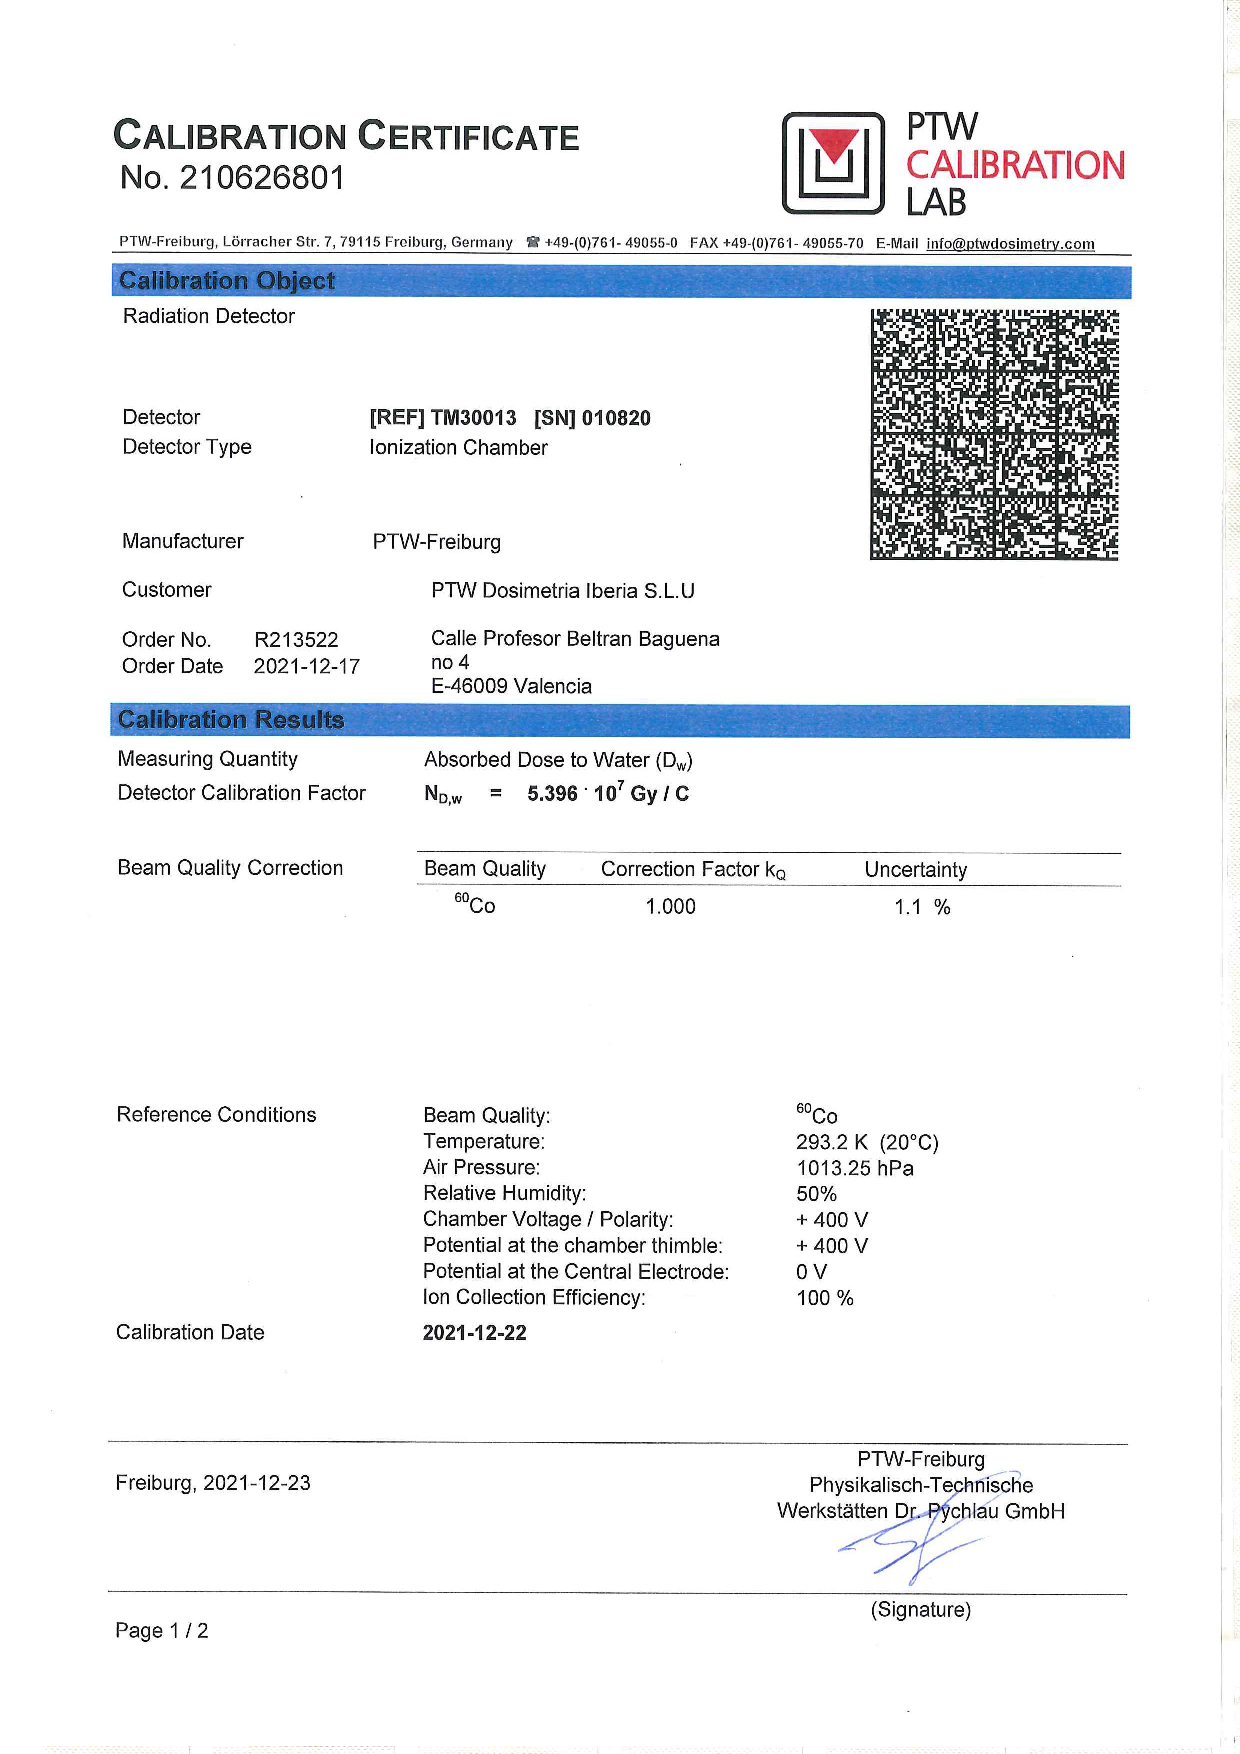
\includepdf[pages=-]{CamaraFarmer10820.pdf}

\end{document}
